\documentclass{article}

\usepackage{amsmath}
\usepackage{float}

\usepackage{graphicx}
\graphicspath{ {../results/} }

\usepackage[style=numeric, backend=bibtex8]{biblatex}
\addbibresource{citations.bib}

\begin{document}

  \title{Linear Time Generation of Simulated Wireless Sensor Networks with Random Geometric Graphs}
  \author{Luke Wood}
  \maketitle

  \section{Executive Summary}
	Wireless Sensor Networks are likely coming in the near future and are incredibly expensive to develop and test.
	This makes them a great candidate for simulation as a preliminary way to gather data.
	Vlady Ravelomananana and Hichem Kenniche from the University of Paris first explored the concept of using random geometric graphs (RGGs) to attempt to model wireless sensor networks \cite{kenniche2010random}.
	In the aforementioned paper it is proven that randomly generated points is the best way to model the incoming wireless sensor networks.
	In this project I will use RGGs as a way to gather valuable information about how wireless sensor networks will possibly function and communicate.

  \subsection{Introduction and Summary}
	Through a series of three reports	I will be analyzing RGGs in the following ways as an attempt to gain some insight into the behavior of wireless sensor networks:
	\begin{enumerate}
		\item Generating RGGs on the geometries of a unit square, unit disc, and unit sphere
		\item Color the generated graph in linear time using smallest vertex last ordering
		\item Find the terminal clique in the generated RGGs
		\item Find a selection of bipartite subgraphs producted by an algorithm for coloring
	\end{enumerate}
	This report is the first of the series and  will describe an implementation for a linear time algorithm to generate graphs consisting of N vertices with an average degree of A on the geometric topologies of: unit square, unit disc, unit sphere.

	\begin{center}
	  \begin{table}[H]
			\begin{tabular}{ |c|c|c|c|c|c| }
				\hline
				Nodes & Expected Avg. Deg. & Real Avg. Deg. & Max Deg. & Min Deg. & Seconds \\
				\hline
				1000 & 64 & 57.568000 & 82 & 10 & 0.279913 \\
				\hline
				5000 & 64 & 60.658400 & 87 & 15 & 0.840636 \\
				\hline
				25000 & 64 & 62.504080 & 98 & 11 & 3.828407 \\
				\hline
				50000 & 64 & 62.986840 & 100 & 20 & 8.938070 \\
				\hline
				100000 & 64 & 63.258520 & 102 & 18 & 14.938207 \\
				\hline
			\end{tabular}
			\caption{Data on graphs generated with the square topology}
		\end{table}
	\end{center}

  Currently, my implementation has support for:
  \begin{enumerate}
		\item Generating a RGG with a unit square topology
		\item Generating a RGG with a unit disc topology
		\item Converting that RGG to an Adjacency List
		\item Serializing Adjacency Lists to files
  \end{enumerate}
  Being able to serialize the Adjacency Lists to files is a noteworthy feature as if there are algorithms that require faster runtimes than a dynamically typed language can support (such as python) we can still generate the RGGs from the generation implementation  and use them in other computation ecosystems.

  \subsection{Programming Environment Description}
		The implementation of the algorithm used to gather the data supporting this report was gathered on a 15 inch Macbook pro 2017 with a 2.9 GHz Intel Core i7 processor and 16 GB of RAM.
		The computer is running macOS High Sierra.
		The graph generation is written in python 3 as generating and connection a graph is not super computationally expensive with even decently large inputs such as 100000.
		The later algorithms may be implemented in a different language such as Elixir to get high levels of concurrency and higher efficiency due to type inference (as opposed to pythons dynamic typing).
  \section{Reduction to Practice}
		In this section I will discuss how the transition from theory to implementation went.  
		I will discuss optimizations I made as well as optimizations that I was aware that I could make but decided not to for reasons.
	\subsection{Data Structure Design}
		In the generation portion of this project I use several different data structures.
		The first one is a python object of custom type node.
		This basically serves as a tuple of values consisting of an X location, a Y location, a list of nodes, and a node number.
		All of these are used during the connecting of the nodes in graph generation excluding node number.
		Node number is assigned during object construction time and is only used when converting the list of nodes into an adjacency list.
		This data structure could be used interchangeably with a statically indexed tuple instead of an object to avoid any overhead associated with objects in python, however I believe that the readability gained from using a custom node class heavily outweighs the marginal performance benefit gained from using a statically indexed tuple.
		Both of these data structures provide $O(1)$ read and write operations.
		If we were to generate gigantic graphs then an argument could be made to switch over the statically indexed tuples to reduce the access time for attributes by a bit.

		The second mentioned data structure is the adjacency list.
		Adjacency lists are an efficient graph representation that we will use in the subsequent reports.
		Adjacency lists require only $O(v*e)$ storage as opposed to the $O(v^2)$ required for adjacency matrixes.
		This is handy in situations where the expected average number of edges is significantly lower than the number of nodes in the graph.
		Despite the huge potential savings on storage, the only sacrifice adjacency lists make is in the lookup operation to determine if there is an edge between two nodes.
		This takes $O(e)$ in an adjacency list as opposed to $O(1)$ in an adjacency matrix.

	\section{Algorithm Description}
		In this section I will give a detailed analysis of the algorithms used in this project.
		I will discuss the runtimes of each algorithm in terms of $\Omega$, $O$, and $\Theta$ when relevant.
  \subsection{Square Point Generation}
		The algorithm to generate the points in the unit square topology is incredibly simple.
		Simply pick two random numbers between 0 and 1 for all nodes.

	\begin{center}
		\begin{table}
			\begin{tabular}{ |c|c|c|c| }
				\hline
				Algorithm & $\Omega$ & $O$ & $\Theta$ \\
				\hline
				Square Point Generation & $\Omega(n)nn$  & & \\
				\hline
				Disc Point Generation & & & \\
				\hline
				Node Connection & & & \\
				\hline

			\end{tabular}
		\end{table}
	\end{center}

  \subsection{Disc Point Generation}
		Generating the points on the Disc topology is slightly more challenging than generating the points for the square topology.
		Instead of picking two numbers between 0 and 1, we apply the following formulae:
  	\begin{center}
    $\theta=rand()$ \newline
    $x=sin(\theta)$ \newline
    $y=cos(\theta)$ \newline
  	\end{center}
		By using the same theta to determine the x and y coordinate we ensure that our points will never fall out of the unit disc.
		I found a formula to generate points on a unit disk using \cite{40023}

		\subsection{Node Connection}
		In order to ensure that average degree of the nodes is close to the desired average degree we define a radius surrounding each node.
		The formulas to find the radius for each topology is derived from the equations found in the paper Bipartite Grid Partitioning of a Random Geometric Graph\cite{chen2017bipartite}.
		The formula used to find this radius varies for each graph tolopogy and can be found in the table displayed below:

		\begin{tabular}{ |c|c|c| }
				\hline
				Topology & Equation Used to Derive Radius & Radius Equation \\
				\hline
				Unit Square & $d(G) \approx N\pi r^2 $ & $r = sqrt(\dfrac{d(G)}{N\pi})$ \\
				\hline
				Unit Disc & $r = sqrt(\dfrac{d(G)}{N\pi})$ & $r = sqrt(\dfrac{d(G)}{N})$ \\
				\hline
				Unit Sphere & & \\
				\hline
		\end{tabular}

		To derive the disc radius formula, I simply multiplied the unit square formula by pi because that is the amount of extra area that the unit disc has over the unit square

		\subsection{Conversion From Node List to Adjacency Matrix}
		The algorithm to convert from a list of the node class I defined to an adjacency list is extremely straight forward.
		The algorithm consists of a pair of nested map operations.
		The first operation maps each node to it's edges list.
		The second operation maps each item of the edge lists to it's respective node number.
		This quickly yields an $O(v*e)$ algorithm to change my node list to an adjacenecy matrix.
		If the performance of $O(v*e)$ is deemed unacceptable in the future, then we can simply append the node number to the list of edges as opposed to a pointer to the node object deeming the second map operation unneccesary yieling an $O(v)$ algorithm.


	  \subsection{Algorithm Engineering}
	  Originally I had a brute force algorithm that ran in $O(n^2)$ time.
	  This quickly became problematic as the algorithm took upwards of 200 seconds to run on input size of only 12,000.
	  \begin{figure}[H]
		\centering
		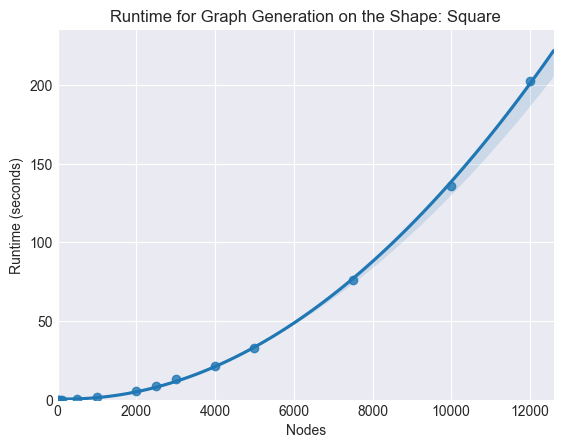
\includegraphics[width=1 \textwidth]{square/runtime/runtime_chart_naive}
		\caption{Runtimes of the $O(n^2)$ Algorithm}
	  \end{figure}


	  To fix this, I overhauled the algorithm to be $O(n)$.
	  I did this by implementing the cell method described above in the Algorithm Description section as well as in Chen's paper Bipartite Grid Partitioning of a Random Geometric Graph\cite{chen2017bipartite}.
	  \begin{figure}[H]
		\centering
		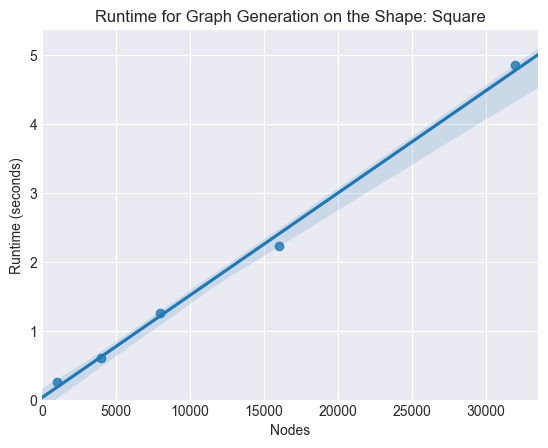
\includegraphics[width=1 \textwidth]{square/runtime/runtime_chart}
		\caption{Runtimes of the $O(n)$ Algorithm}
	  \end{figure}

	  I have also included a table to compare some of the runtimes for the same size inputs below.

	  \begin{center}
	  \begin{table}[H]
		\begin{tabular}{ |c|c|c| }
			\hline
			Nodes & $O(n^2)$ & $O(n)$ \\
			\hline
			  1000 & 0.258400 & 0.657174 \\
			  \hline
			  2000 & 0.382116 & 2.630040 \\
			  \hline
			  3000 & 0.473916 & 5.874501 \\
			  \hline
			  5000 & 0.831753 & 16.809004 \\
			  \hline
			  10000 & 1.560216 & 65.398991 \\
			\hline
		\end{tabular}
		\caption{Runtimes of the $O(n)$ and $O(n^2)$ algorithms in seconds}
	  \end{table}
	  \end{center}

	  The $O(n)$ algorithm is far superior even on small input sizes such as 1000.

	\subsection{Verification}
		One way that we verified our results was checking the distribution of edge densities in our graph.
		We expect to see a gaussian distribution in the edge densities with the center being around our calculated radius.
		We can also verify the runtime of our algorithms by plotting the input size on the x axis and the runtime on the y axis.
		If we have a linear algorithm we should be able to fit the distribution of points to a linear equation with minimal error.
		Both of these verification methods were successful and can be seen in the results section of this report.

\section{Result Summary}
  \subsection{Edge Density}
  As expected I got a gaussian distribution for my edge densities.
  \begin{figure}[H]
  \centering
  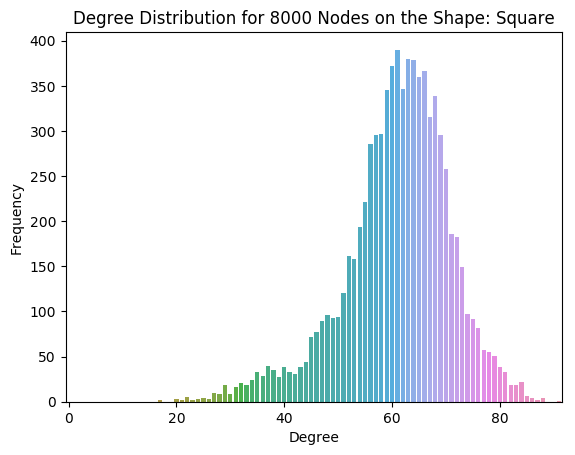
\includegraphics[width=1 \textwidth]{square/edge_density/8000_64.png}
  \caption{Edge Densities of an 8000 Node Graph with E(Degree)=64}
  \end{figure}

  \subsection{Performance Rates}
  \begin{center}
	  \begin{table}[H]
		  \begin{tabular}{ |c|c|c| }
			\hline
			Nodes & Topology & Runtime \\
			\hline
		  \end{tabular}
		  \caption{Runtimes of the $O(n)$ vertex connection algorithm}
	  \end{table}
  \end{center}

\printbibliography

\end{document}
